% ========================================================
% -------------------- Orca Method ----------------------
% ========================================================

\section{Orca}\label{sec:method}
\setnavsection{sec:method}


\subsection{Modeling}
\label{sec:method_modeling}


\paragraph{Macro.} Orca formulates world learning as latent world-state modeling, including state abstraction from multimodal world signals and state transition.
Given the world signals $\mathcal{X}, \mathcal{X}=\{X^{m}\}_{m\in\mathcal{M}}$, where $\mathcal{M}$ can encompass a rich variety of modalities. Ideally, $\mathcal{X}$ should include all signals present in the world, such as \textit{common multimodal signals}: language, vision, and audio; \textit{physical signals}: force and light; and even \textit{signals beyond human perception}: infrared radiation. Mapping $\mathcal{X}$ to a latent world state $\mathcal{S}$, i.e., $\mathcal{S} = f_{\theta}(\mathcal{X}).$
We model the state $S\in \mathcal{S}$ evolves forwards and backwards under \textit{implicit dynamics} and \textit{explicit conditions}:
\begin{equation}
\label{eq:Orca_state_transition}
    S_{t+\Delta}\sim p_{\Theta}
    \left(S_{t+\Delta}\mid S_t,z_t,c_t\right),
    \quad \Delta\in\mathbb{Z}_{\ne 0}.
\end{equation}
where, $z_t$ is a way to realize \textit{invisible dynamics}. It captures latent or unobserved factors that drive state changes, such as physical laws, object properties, scene dynamics, and environmental forces. $c_t$ is a way to realize \textit{explicit conditions}. It refers to observed conditions such as human instructions. $\Delta>0$ represents predicting future states $S_{> t}$, while $\Delta<0$ represents backtracking to past states $S_{< t}$. 



\paragraph{Details.} 
In this version, Orca uses visual signals and language signals as two fundamental types of multimodal world signals.
To realize the state-transition modeling in Equation~\ref{eq:Orca_state_transition}, Orca adopts two complementary learning paradigms: \textit{unconscious learning} and \textit{conscious learning}.



\vspace{-1ex}
\begin{enumerate}[label={}, leftmargin=10pt, itemindent=0pt, itemsep=0.3em, topsep=0.3em]

    \item[] \textit{\textbf{1) Unconscious learning} learns state transitions from observation alone.} \ The model observes naturally occurring transitions without explicit semantic conditions. It can learn how objects move, natural dynamics, physical regularities, or how scenes transition over time. This is equivalent to $c_t=\varnothing$, i.e., $S_{t+\Delta}\sim p_{\Theta}^{\mathrm{u}}\left(S_{t+\Delta}\mid S_t,z_t\right)$. In this paradigm, the target state originates from the nearest future observation.
    \textit{Unconscious learning} can learn dense and natural state transitions.


    \item[] \textit{\textbf{2) Conscious learning} learns state transitions under explicit semantic conditions.} \ Given a language signal, Orca treats it as an explicit condition that guides the state transition. The language condition can specify an event $c_t=e_{t+\Delta}$, including a future or past event, i.e., $S_{t+\Delta}\sim p_{\Theta}^{\mathrm{c}}(S_{t+\Delta}\mid S_t, z_t,e_{t+\Delta})$. The condition can also be a task intention or a causal premise. It guides how the current state should transition toward a target state. \textit{Conscious learning} can learn sparse and meaningful state transitions.

\end{enumerate}



\subsection{Architecture}
\label{sec:method_architecture}


\begin{figure}[!htbp]
    \centering
    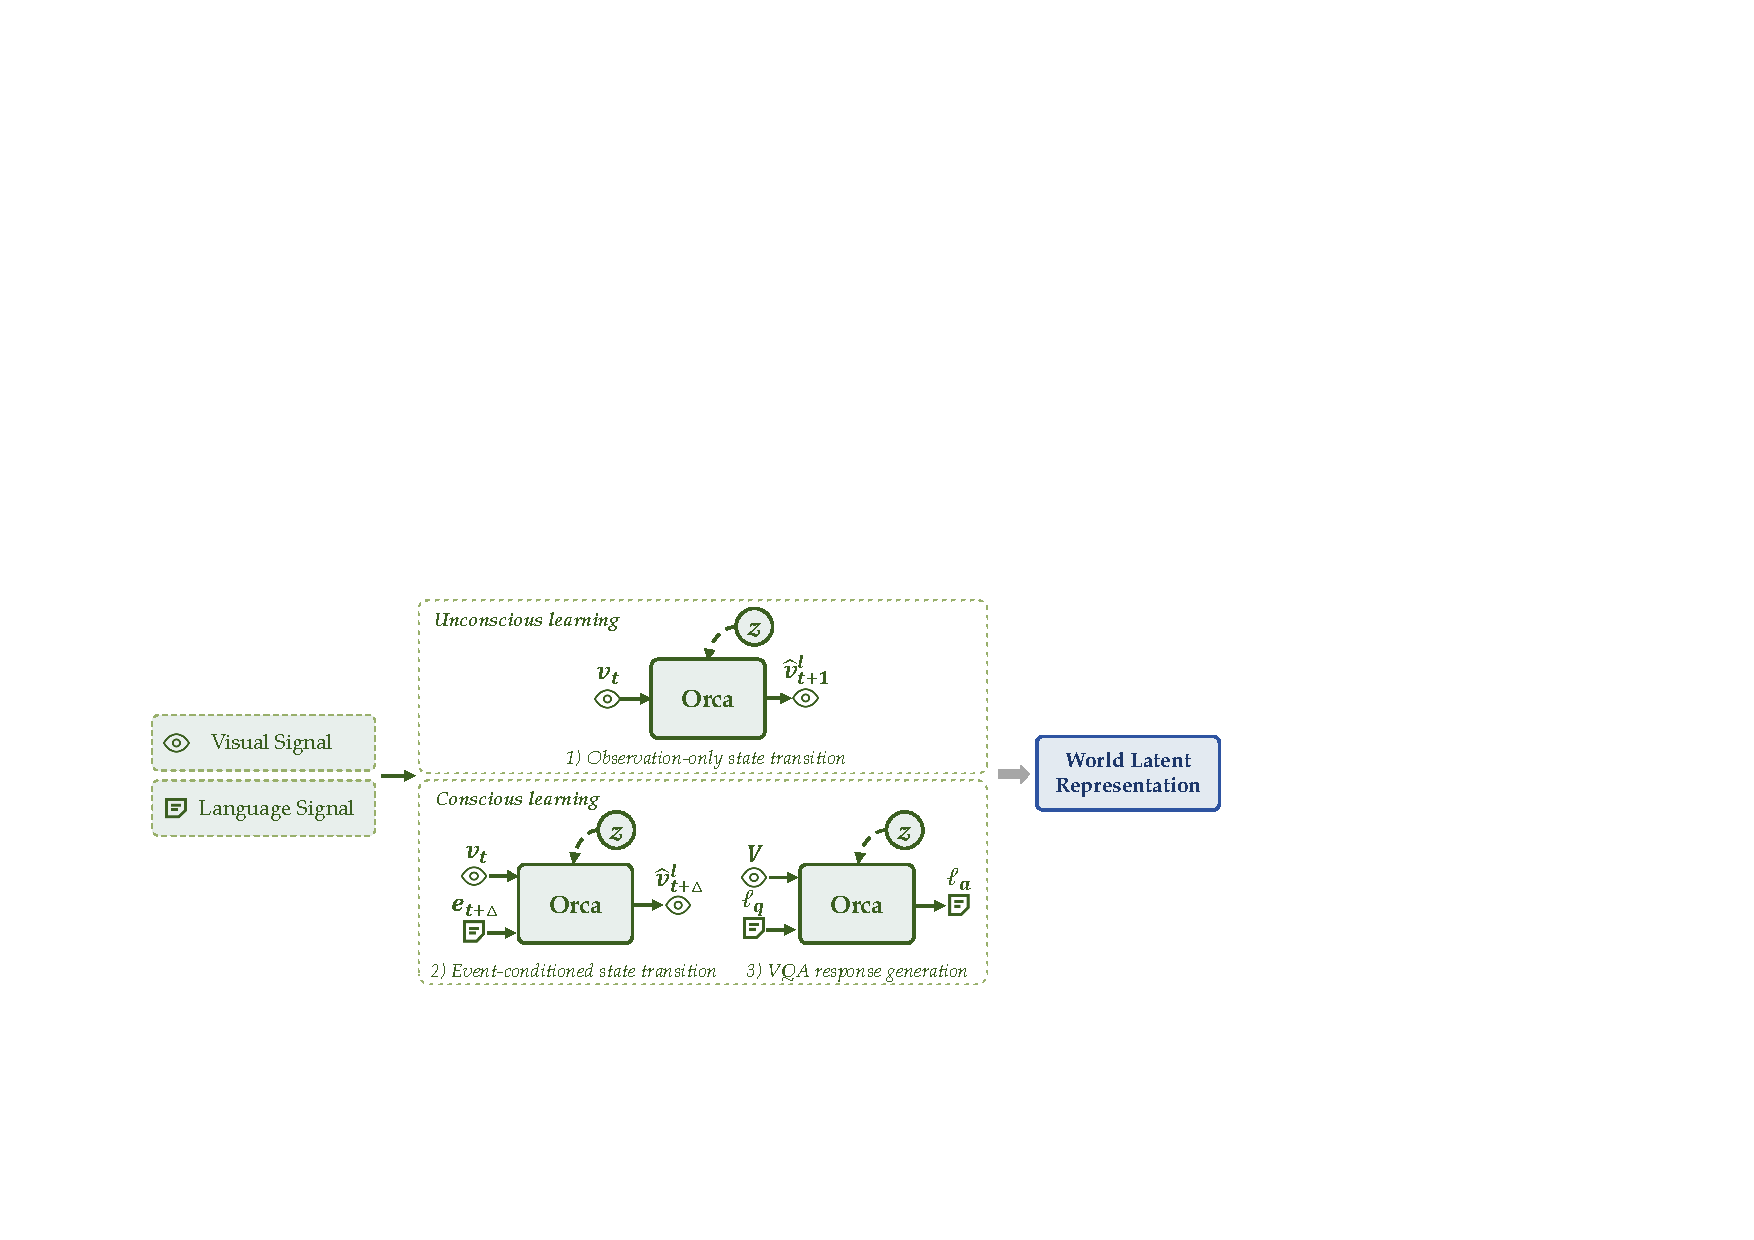
\includegraphics[width=1\linewidth]{figs/method/method_Orca.pdf}
    \caption{\textbf{Overview of Encoder.} Orca learns a world latent representation through two learning paradigms. \textit{Unconscious learning} uses video data to capture dense and natural state transitions. \textit{Conscious learning} uses language instructions as explicit semantic conditions to capture sparse and meaningful state transitions.}\label{fig:Orca_architecture}
    \vspace{-0.5em}
\end{figure} 

\paragraph{Encoder.} 
Orca focuses on the \textit{\textbf{Encoder}}, which learns a unified world latent space for state abstraction and state transition.
The overview of the \textit{\textbf{Encoder}} is shown in Figure \ref{fig:Orca_architecture}. It uses a native pre-trained VLM \citep{qwen35} aligned with the language and vision spaces. Given visual and language signals, Orca learns the world latent through \textit{unconscious learning} and \textit{conscious learning}.

The input of \textit{unconscious learning} is a certain frame $v_t$ of the video $V$, and the output is the prediction latent $\hat{v}^l_{t+1}$ of the next adjacent frame. After passing through the VLM, $v_t$ will be used to obtain the predicted $\hat{v}^l_{t+1}$ through two layers of MLP. The ground truth of the next adjacent frame $v_{t+1}$ will only pass through the frozen vision encoder to obtain a latent representation $v^l_{t+1}$, and then be teacher forced with the prediction latent $\hat{v}^l_{t+1}$. This part completes the \textit{1) Observation-only state transition} in Figure \ref{fig:Orca_architecture}.

To support \textit{conscious learning}, we divide the video into multiple segments based on meaningful events. Each event contains a video segment and a corresponding instruction description, as shown in \textbf{Section \ref{sec:pretraining_data}}. The input of \textit{conscious learning} also includes a frame $v_t$ from $V$, along with an instruction description $e_{t+\Delta}$ of the adjacent (next or previous) event, where $v_t$ belongs to a certain event. The output is the prediction latent $\hat{v}^l_{t+\Delta}$ of a random sample associated with the event $e_{t+\Delta}$. This part completes the \textit{2) Event-conditioned state transition} in Figure \ref{fig:Orca_architecture}. In addition, the essence of conscious learning is understanding the world. Therefore, we will also input the video $V$ and the related questions $l_q$, and output the corresponding language answers $l_a$. This part completes the \textit{3) VQA response generation} in Figure \ref{fig:Orca_architecture}. Ultimately, the world latent space is obtained by the two learning paradigms. 

\paragraph{Decoder.} The learned latent space is read out by the modality-specific \textbf{\textit{Decoder}} to extract multi-modal information. Since the decoder is not the focus of this section, its details will be shown in \textbf{Section \ref{sec:downstream_readout}.}

